%%%%%%%%%%%%%%%%%%%%%%%%%%%%%%%%%%%%%%%%%
% baposter Landscape Poster
% LaTeX Template
% Version 1.0 (11/06/13)
%
% baposter Class Created by:
% Brian Amberg (baposter@brian-amberg.de)
%
% This template has been downloaded from:
% http://www.LaTeXTemplates.com
%
% License:
% CC BY-NC-SA 3.0 (http://creativecommons.org/licenses/by-nc-sa/3.0/)
%
%%%%%%%%%%%%%%%%%%%%%%%%%%%%%%%%%%%%%%%%%

%----------------------------------------------------------------------------------------
%	PACKAGES AND OTHER DOCUMENT CONFIGURATIONS
%----------------------------------------------------------------------------------------

\documentclass[landscape,paperwidth=58in,paperheight=40in,fontscale=0.285]{baposter} % Adjust the font scale/size here

\usepackage{graphicx} % Required for including images
\graphicspath{{fig/}} % Directory in which figures are stored

\usepackage{amsmath} % For typesetting math
\usepackage{amssymb} % Adds new symbols to be used in math mode

\usepackage{booktabs} % Top and bottom rules for tables
\usepackage{enumitem} % Used to reduce itemize/enumerate spacing
\usepackage{palatino} % Use the Palatino font
\usepackage[font=small,labelfont=bf]{caption} % Required for specifying captions to tables and figures

\usepackage{multicol} % Required for multiple columns
\setlength{\columnsep}{1.5em} % Slightly increase the space between columns
\setlength{\columnseprule}{0mm} % No horizontal rule between columns

\usepackage{tikz} % Required for flow chart
\usetikzlibrary{shapes,arrows} % Tikz libraries required for the flow chart in the template

\newcommand{\compresslist}{ % Define a command to reduce spacing within itemize/enumerate environments, this is used right after \begin{itemize} or \begin{enumerate}
\setlength{\itemsep}{1pt}
\setlength{\parskip}{0pt}
\setlength{\parsep}{0pt}
}

\definecolor{lightblue}{rgb}{0.145,0.6666,1} % Defines the color used for content box headers

\usepackage{enumitem}
\usepackage{amsfonts}
\usepackage{tipa}  % Packages for IPA symbols
\let\ipa\textipa
\usepackage{color}

\begin{document}

\begin{poster}
{
headerborder=closed, % Adds a border around the header of content boxes
colspacing=1em, % Column spacing
bgColorOne=yellow!20, % Background color for the gradient on the left side of the poster
bgColorTwo=yellow!20, % Background color for the gradient on the right side of the poster
borderColor=orange, % Border color lightblue
headerColorOne=black, % Background color for the header in the content boxes (left side)
headerColorTwo=lightblue, % Background color for the header in the content boxes (right side)
headerFontColor=white, % Text color for the header text in the content boxes
boxColorOne=white, % Background color of the content boxes
textborder=roundedleft, % Format of the border around content boxes, can be: none, bars, coils, triangles, rectangle, rounded, roundedsmall, roundedright or faded
eyecatcher=true, % Set to false for ignoring the left logo in the title and move the title left
headerheight=0.1\textheight, % Height of the header
headershape=roundedright, % Specify the rounded corner in the content box headers, can be: rectangle, small-rounded, roundedright, roundedleft or rounded
headerfont=\Large\bf\textsc, % Large, bold and sans serif font in the headers of content boxes
%textfont={\setlength{\parindent}{1.5em}}, % Uncomment for paragraph indentation
linewidth=2pt % Width of the border lines around content boxes
}
%----------------------------------------------------------------------------------------
%	TITLE SECTION 
%----------------------------------------------------------------------------------------
%
{\includegraphics[height=0.07\textwidth, width=0.05\textwidth]{imark_1867_bold.png}} % First university/lab logo on the left
{\bf\textsc{An Investigation On Training Deep Neural Networks Using Probabilistic Transcriptions}\vspace{0.1em}} % Poster title
{\textsc{Amit Das, Mark Hasegawa-Johnson}\\\hspace{5pt}\textsc{Dept. of ECE \& Beckman Institute, University of Illinois, USA}} % Author names % Institution
{\vspace{-1em}\includegraphics[width=0.20\textwidth, height=0.035\textwidth]{BeckmanLogo}}% Second university/lab logo on the right

%----------------------------------------------------------------------------------------
%	OBJECTIVES
%----------------------------------------------------------------------------------------

\headerbox{1. Objectives}{name=objectives,column=0,row=0}{

How do we train DNNs (Deep Neural Networks) using \textcolor{red}{\textbf{noisy transcriptions}} collected from \textcolor{red}{\textbf{non-native crowd workers}} on the web? These workers do not speak the native/target language. Hence, the transcriptions they provide are prone to labeling errors. Standard DNN training using such transcriptions do not yield significant improvements over GMM-HMM systems.\\

\textbf{Main Contributions:} 
\begin{itemize}[label={\checkmark}]\compresslist
\item Investigate DNN training methods effective for training using non-native crowd transcriptions.
\item Achieved consistent and absolute improvement in PERs (phone error rates) in the range 1.3-6.2\% over GMM-HMM.
\end{itemize}

\vspace{0.3em} % When there are two boxes, some whitespace may need to be added if the one on the right has more content
}

%----------------------------------------------------------------------------------------
%	MOTIVATION
%----------------------------------------------------------------------------------------

\headerbox{2. Motivation}{name=motivation,column=0,below=objectives}{

\begin{itemize}
\item Rich resourced languages (e.g. English) have $>$100 hours of labeled data and $>$100k entries in their lexicon. This is the typical requirement to build good ASR systems.
\item For under-resourced languages, it is possible to find speech waveforms and text data but hard to find corresponding labels for those waveforms.
\item In the absence of native transcripts, we resort to collecting \textit{approximate} transcripts collected
from non-native crowd workers. And, train ASR systems using these transcripts.
\end{itemize}
}


%----------------------------------------------------------------------------------------
%	REFERENCES
%----------------------------------------------------------------------------------------

\headerbox{References}{name=references,column=0,span=2,above=bottom}{

\renewcommand{\section}[2]{\vskip 0.05em} % Get rid of the default "References" section title
\nocite{*} % Insert publications even if they are not cited in the poster
\small{ % Reduce the font size in this block
[1] M. Hasegawa-Johnson \textit{et al.}, ``ASR for Under-Resourced Languages from Probabilistic Transcription," IEEE Trans. Audio Speech \& Lang. Proc. (under review).
%\bibliographystyle{unsrt}
%\bibliography{sample.bib} % Use sample.bib as the bibliography file
}
}


%----------------------------------------------------------------------------------------
%	SCENARIO
%----------------------------------------------------------------------------------------

\headerbox{3. Scenario}{name=scenario,column=0,below=motivation,above=references}{

\begin{center}
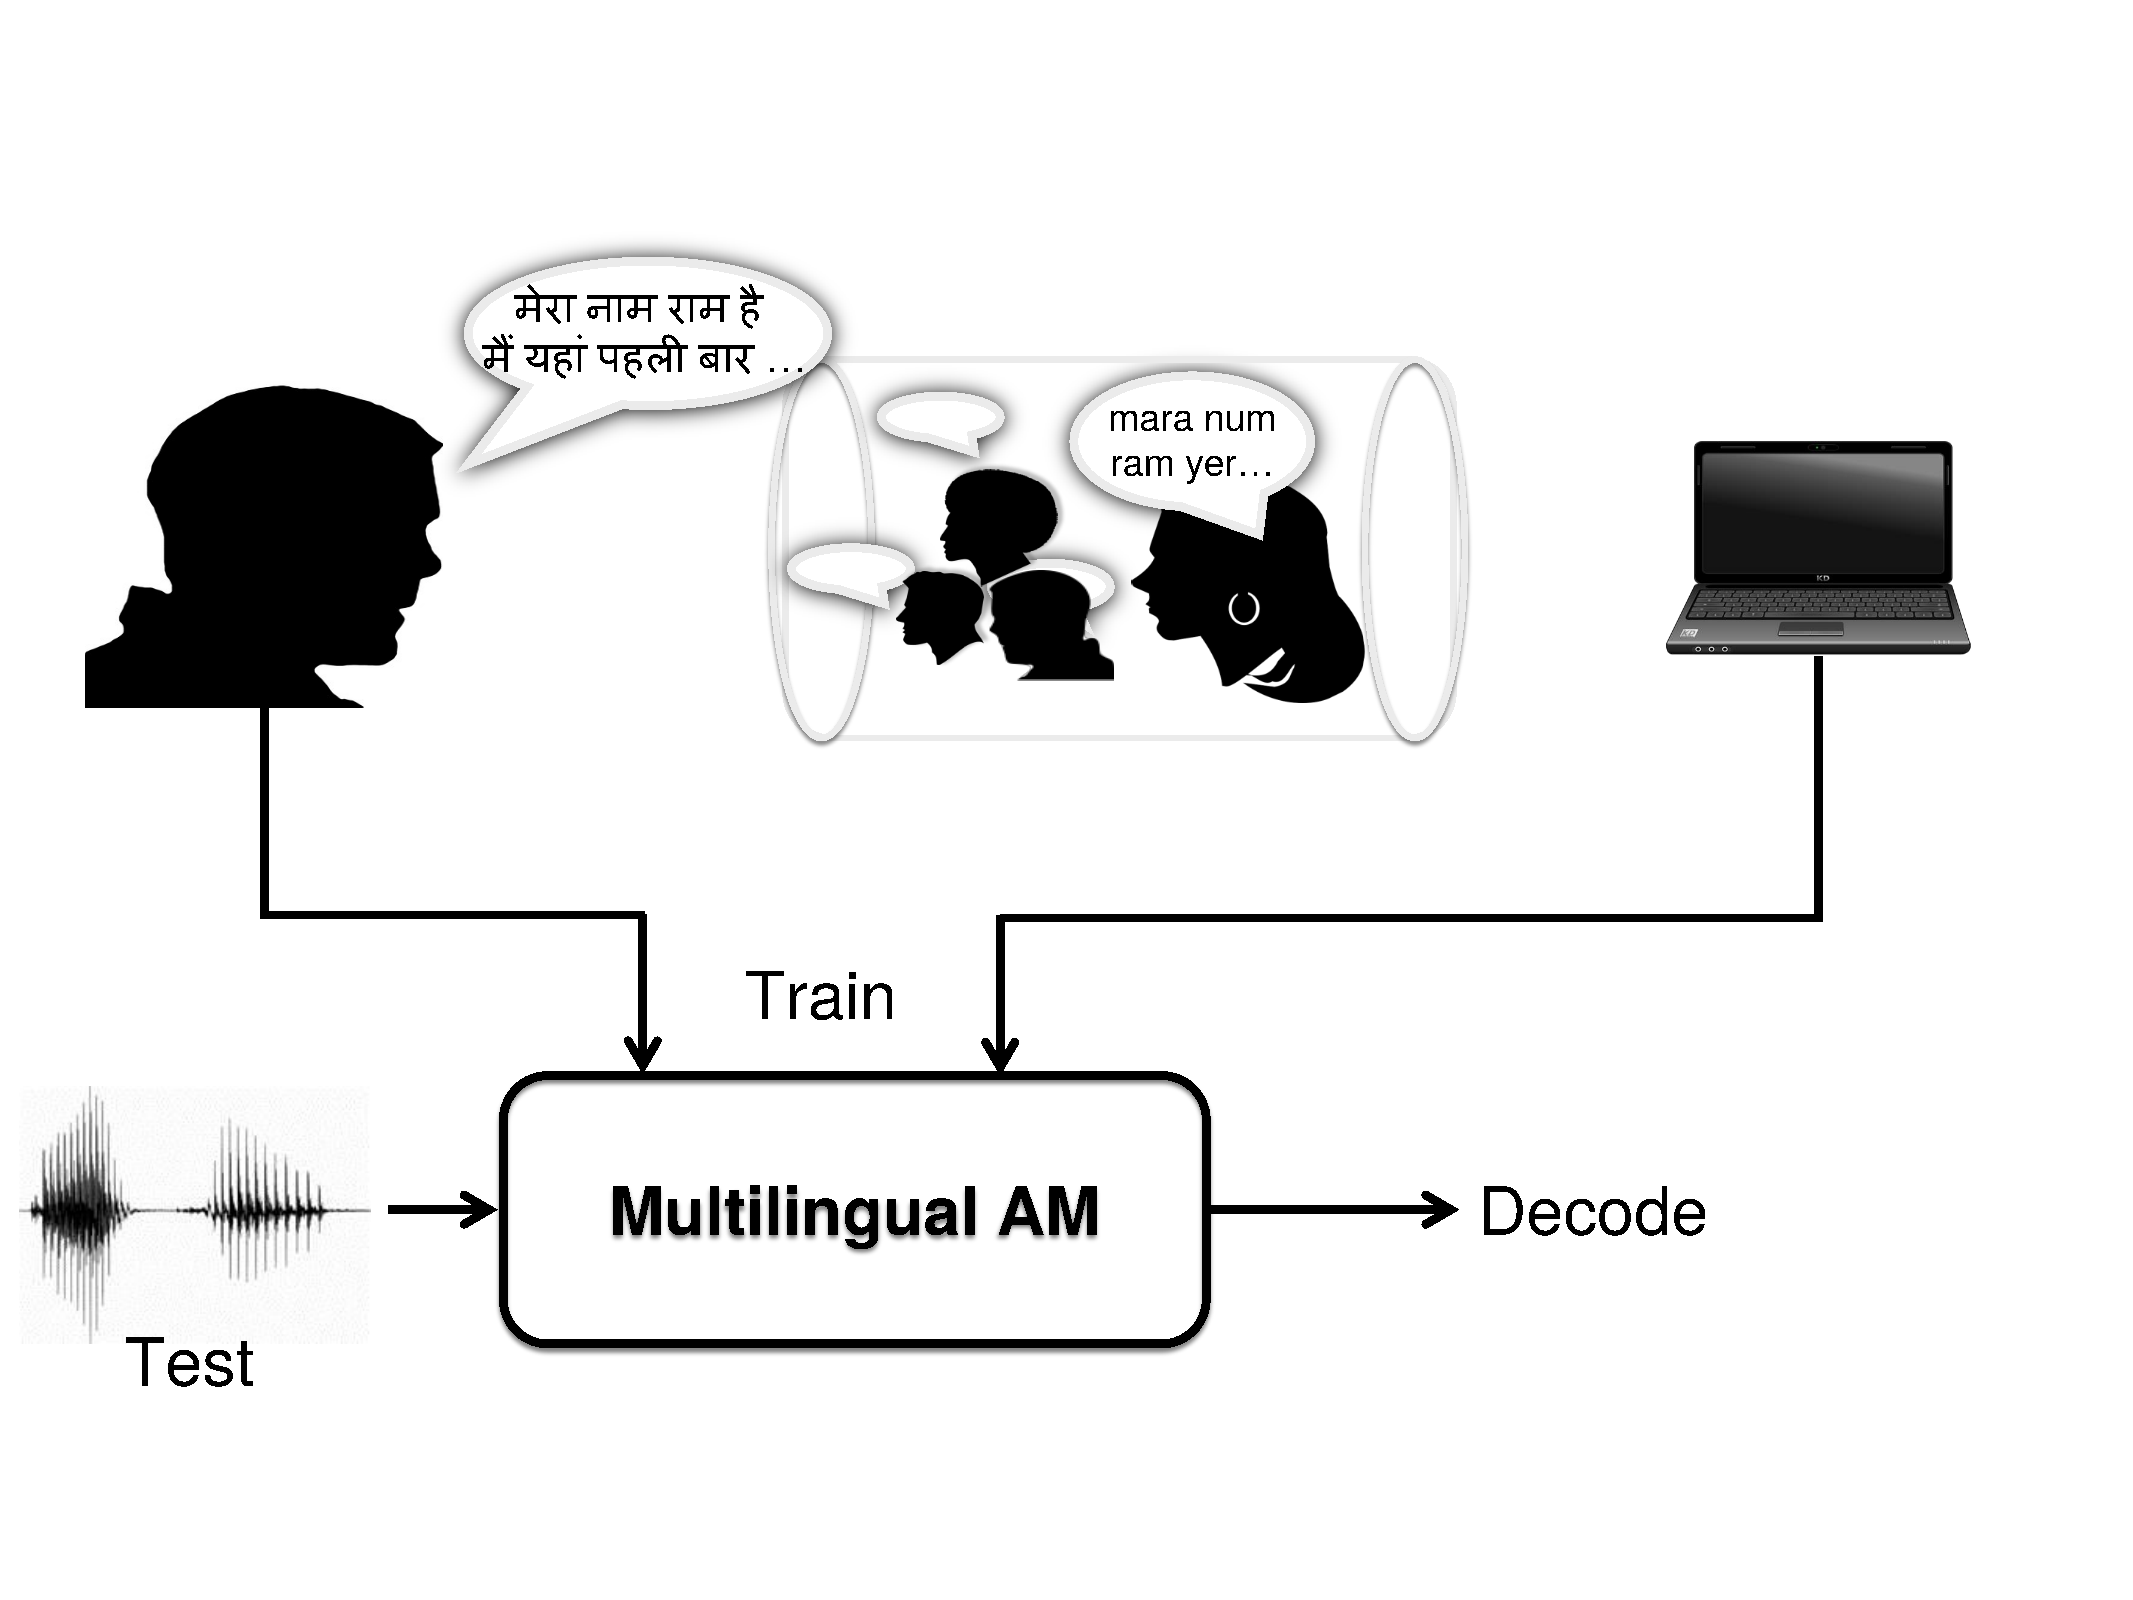
\includegraphics[width=0.9\textwidth, height=0.55\linewidth,trim=0mm 0mm 25mm 40mm, clip]{mc_flowchart.pdf}
\end{center}
\vspace{-15mm}
\begin{itemize}
 \item We do \textcolor{red}{\underline{not}} have natively transcribed labeled data in the target language $\textbf{L}$. Transcripts from native transcribers are called \textbf{DTs} (\textbf{deterministic transcripts}).
\item We have non-natively transcribed labeled data from crowd workers who neither speak nor have any familiarity with $\textbf{L}$. Hence, these transcripts are prone to labeling errors. Transcripts from crowd workers are called \textbf{PTs} (\textbf{probabilistic transcripts}). 
\end{itemize}

}


%----------------------------------------------------------------------------------------
%	DT vs PT
%----------------------------------------------------------------------------------------

\headerbox{4. DT vs PT}{name=dtvspt,column=1,row=0,aligned=objectives}{

\begin{center}
\includegraphics[width=0.9\textwidth]{DTvsPT}
\end{center}


\begin{center}
    %\begin{tabular}{ | l | l | l | p{5cm} |}
    \begin{tabular}{ l | l  l  }
    \hline
     & DT & PT  \\ \hline
    Transcribers & Native & Crowdworkers \\
    Transcription Structure & Single stream  &  Lattice \\
    Probability & $1.0$  & $(0, 1]$ \\
    Label Noise & Low & High \\
    Availability  & Difficult & Easy \\
    \hline
    \end{tabular}
\end{center}

}

%----------------------------------------------------------------------------------------
%	CORPUS
%----------------------------------------------------------------------------------------
\headerbox{5. Corpus}{name=corpus,column=1,below=dtvspt,bottomaligned=scenario}{

\begin{center}
\captionof{table}{SBS Multilingual Corpus ($\approx$ 40 min per language)}
\begin{tabular}{l|c c| c}
   \hline
Language &  \multicolumn{2}{c|}{Utterances}  & Phones \\
                 &  Train & Test &  \\ \hline
Swahili (SW)     & 463 & 123 & 53 \\
Hungarian (HG)    & 459 & 117 & 70 \\
Cantonese (CA)  & 544 & 148 &  37 \\
Mandarin (MD) & 467 & 113 &  57 \\
Arabic (AR) & 468 & 112 &  51 \\
Urdu (UR) & 385 & 94 &  45 \\ \hline
All & - & - & 83 \\ \hline
\end{tabular}
\end{center}

\begin{itemize}
\item We pick a language as the test/target language, $\textbf{L}$, from the above table.
\item Then training data for $\textbf{L}$ are:
\begin{itemize}
\item PTs in $\textbf{L}$. But we do not include DTs in $\textbf{L}$.
\item DTs in all the other languages ($\ne \textbf{L}$).
\item Any unlabeled data that might be available in $\textbf{L}$.
\end{itemize}
\end{itemize}

\textbf{Example: Swahili as a test langauge}
\vspace{-5mm}
\begin{center}
\captionof{table}{Training data for Swahili}
\begin{tabular}{l|c|c}
   \hline
Language &   Transcript Type & Amount of Data \\ \hline
SW  & PT  & 40 min \\
HG + CA + MD + $\cdots$  & DT & 200 min  \\
AR + UR          &    & (40 min $\times$ 5 lang) \\
SW  & Unlabeled  &  5 hrs \\ \hline
\end{tabular}
\end{center}

\textbf{Note:} DTs in Swahili are never used for training.


}

%----------------------------------------------------------------------------------------
%	DNN TRAINING
%----------------------------------------------------------------------------------------

\headerbox{6. Training DNN Using Probabilistic Transcriptions}{name=dnntraining,column=2,span=2}{

\begin{multicols}{2}
\vspace{1em}
\begin{itemize}
\item Standard DNN cross-entropy training not significantly better (or sometimes worse) than GMM-HMM when trained using PTs.
\item \textbf{Problem:} Discriminative training is sensitive to noise.
\item Example of a frame containing 'ae': (\textcolor{green}{green} = true label, \textcolor{red}{red} = incorrect label) 
\begin{itemize}
\item DT: Train using 1-hot labels $\Rightarrow$ $[1.0 \ \textcolor{green}{\text{\ipa{\ae}}}]$
\item PT: Train using soft labels $\Rightarrow$  $[0.35 \ \textcolor{red}{\text{\ipa{a}}}, 0.45 \ \textcolor{red}{\text{\ipa{5}}},  0.1 \ \textcolor{green}{\text{\ipa{\ae}}}, 0.1 \ \textcolor{red}{\text{\ipa{E}}}]$
\end{itemize}
\item \textbf{Solution:} \textbf{Transfer knowledge from DT to PT using Multi-task Learning (MTL).}
\begin{itemize}\compresslist
\item Train PT and DT using two different softmax layers.  Or, train using PT, DT and ST (self-training transcripts) in three different softmax layers.
\item DT and high confidence STs help fix the errors in hidden layers. Obtain better feature separation in the hidden layers.
\end{itemize}
\end{itemize}

\begin{center}
\includegraphics[width=0.48\textwidth,height=0.7\linewidth]{DNN_multisoftmax}
\captionof{figure}{(a) DNN-1 (No MTL),  (b) DNN-2 (MTL),  (c) DNN-3 (MTL)}
\end{center}
\end{multicols}


}


%----------------------------------------------------------------------------------------
%	RESULTS
%----------------------------------------------------------------------------------------

\headerbox{7. Results}{name=results,column=2,span=2,below=dnntraining}{

\begin{multicols}{2}
\vspace{1em}
\textbf{Best Case PER}\vspace{-2mm}
\begin{itemize}
\item [\checkmark] DTs available in the target language (Oracle scenario); Monolingual training.
\end{itemize}

\begin{center}
\captionof{table}{MONO (Dev set PER inside parentheses)}
\begin{tabular}{l|c c}
   \hline
Lang  & \multicolumn{2}{c}{PER (\%)} \\
          & HMM     & DNN   \\ \hline
SW        & 35.63 (47.00)   & 34.18 (39.49)   \\
HG        & 38.72 (40.33)   & 35.62 (37.32)   \\
MD        & 31.80 (26.14)   & 28.26 (25.16)   \\ \hline
\end{tabular}
\end{center}

\vfill
\columnbreak
\textbf{Worst Case PER}\vspace{-2mm}
\begin{itemize}\compresslist
\item [{$\times$}] DTs not available in the target language.
\item [{$\times$}] PTs not available in the target language.
\item [{$\checkmark$}] DTs available in other languages; Multilingual training.
\end{itemize}

\begin{center}
\captionof{table}{MULTI (Dev set PER inside parentheses)}
\begin{tabular}{l|c c c}
   \hline
Lang  & \multicolumn{3}{c}{PER (\%)} \\
          &  HMM & DNN & \# Senones   \\ \hline
SW      &65.73 (67.58)   &61.17 (63.12) & 1003 \\
HG      &67.55 (68.50)   &63.25 (63.65) &  1012 \\
MD     &71.09 (69.10)   &64.68 (63.84) & 994  \\ \hline
\end{tabular}
\end{center}
\end{multicols}


\begin{center}
 \begin{tabular}{@{}l@{}}
    \\ \textbf{PER of Proposed DNNs}\\
    {$\times$}\hspace{2mm} DTs not available in the target language. \\
    {$\checkmark$}\hspace{2mm} PTs available in the target language. \\
    {$\checkmark$}\hspace{2mm} DTs available in other languages.
 \end{tabular}
\end{center}

\vspace{-8mm}
\begin{center}
\captionof{table}{Comparison of PERs of baseline (MULTI, MAP HMM, DNN-1) vs proposed systems (DNN-2, DNN-3). Absolute improvement in PER over MAP HMM in parentheses.}
\begin{tabular}{l|c c c c c c}
\hline
Lang  & \multicolumn{6}{c}{PER (\%)} \\
        &MULTI (Worst) &MAP HMM       &DNN-1    &DNN-2   &DNN-3 &MONO (Best) \\ \hline
SW      &65.73  &44.77  &45.14 (\color{red}\bf{-0.37}) &43.03 ({\color{blue}\bf{1.74}})  &43.50 (1.27) & 35.63   \\
HG      &67.55  &56.85  &56.13 (\color{red}\bf{0.72}) &55.53  ({\color{blue}\bf{1.32}})  &55.69 (1.16)  & 38.72  \\
MD      &71.09  &59.23  &54.95 (4.28) &53.70  (5.53)  &53.05 ({\color{blue}\bf{6.18}})  & 31.80  \\ \hline
\end{tabular}
%\label{Tab:PER_PT}
\end{center}

}


%----------------------------------------------------------------------------------------
%	CONCLUSION
%----------------------------------------------------------------------------------------

\headerbox{8. Conclusions}{name=conclusion,column=2,span=2,below=results,above=bottom}{

\begin{itemize}
\item Proposed DNN-2/DNN-3 systems achieved absolute improvement in PERs in the range 1.3-6.2\% over GMM-HMM systems consistently.
\item They are able to close between 28\% and 67\% (relative) of the gap between MULTI and MONO systems. Thus, PTs are between one and two thirds as useful as DTs.
\item Crowdsourced PTs are not as useful as DTs. The gap between MONO and DNN-2/DNN-3 is still large.
\end{itemize}
}

%----------------------------------------------------------------------------------------

\end{poster}

\end{document}